\documentclass[border=6pt]{standalone}
\usepackage{amsmath,amssymb,tikz}
\usetikzlibrary{arrows.meta,positioning}
\begin{document}
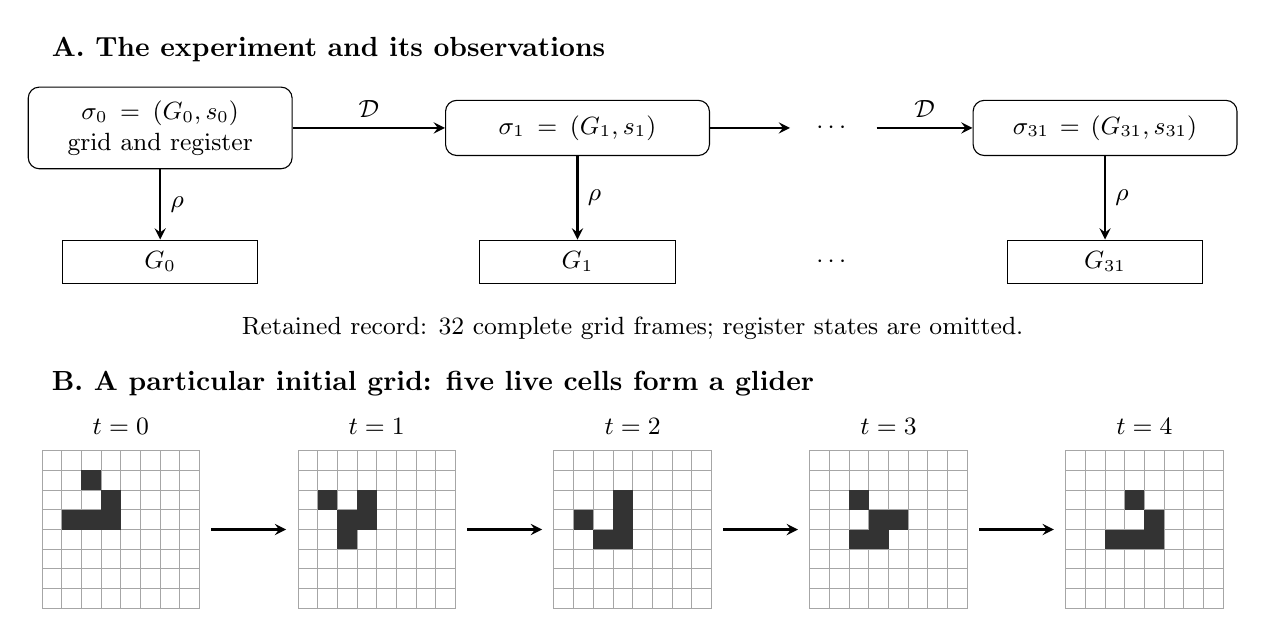
\begin{tikzpicture}[x=1cm,y=1cm,>=stealth,font=\small,
  state/.style={draw,rounded corners,align=center,text width=3.0cm,minimum height=0.7cm,inner sep=5pt},
  frame/.style={draw,align=center,text width=2.2cm,minimum height=0.55cm,inner sep=4pt}]
\node[anchor=west,font=\bfseries] at (0,7.1) {A. The experiment and its observations};
\node[state] (s0) at (1.5,6.1) {$\sigma_0=(G_0,s_0)$\\grid and register};
\node[state] (s1) at (6.8,6.1) {$\sigma_1=(G_1,s_1)$};
\node[state] (slast) at (13.5,6.1) {$\sigma_{31}=(G_{31},s_{31})$};
\draw[->,thick] (s0) -- node[above] {$\mathcal D$} (s1);
\node at (10.05,6.1) {$\cdots$};
\draw[->,thick] (s1.east) -- (9.5,6.1);
\draw[->,thick] (10.6,6.1) -- node[above] {$\mathcal D$} (slast.west);
\node[frame] (g0) at (1.5,4.4) {$G_0$};
\node[frame] (g1) at (6.8,4.4) {$G_1$};
\node[frame] (glast) at (13.5,4.4) {$G_{31}$};
\foreach \a/\b in {s0/g0,s1/g1,slast/glast}{
  \draw[->,thick] (\a.south) -- node[right] {$\rho$} (\b.north);}
\node at (10.05,4.4) {$\cdots$};
\node[align=center] at (7.5,3.55) {Retained record: 32 complete grid frames; register states are omitted.};
\node[anchor=west,font=\bfseries] at (0,2.85) {B. A particular initial grid: five live cells form a glider};
\begin{scope}[shift={(0.0,0)}]
\foreach \i in {0,...,7}{\foreach \j in {0,...,7}{\draw[black!35,line width=0.3pt] (\i*0.25,\j*0.25) rectangle ++(0.25,0.25);}}
\fill[black!80] (0.25,1.0) rectangle ++(0.25,0.25);
\fill[black!80] (0.5,1.5) rectangle ++(0.25,0.25);
\fill[black!80] (0.5,1.0) rectangle ++(0.25,0.25);
\fill[black!80] (0.75,1.25) rectangle ++(0.25,0.25);
\fill[black!80] (0.75,1.0) rectangle ++(0.25,0.25);
\node[anchor=south] at (1,2.08) {$t=0$};
\end{scope}
\draw[->,thick] (2.15,1) -- (3.1,1);
\begin{scope}[shift={(3.25,0)}]
\foreach \i in {0,...,7}{\foreach \j in {0,...,7}{\draw[black!35,line width=0.3pt] (\i*0.25,\j*0.25) rectangle ++(0.25,0.25);}}
\fill[black!80] (0.25,1.25) rectangle ++(0.25,0.25);
\fill[black!80] (0.5,1.0) rectangle ++(0.25,0.25);
\fill[black!80] (0.5,0.75) rectangle ++(0.25,0.25);
\fill[black!80] (0.75,1.25) rectangle ++(0.25,0.25);
\fill[black!80] (0.75,1.0) rectangle ++(0.25,0.25);
\node[anchor=south] at (1,2.08) {$t=1$};
\end{scope}
\draw[->,thick] (5.4,1) -- (6.35,1);
\begin{scope}[shift={(6.5,0)}]
\foreach \i in {0,...,7}{\foreach \j in {0,...,7}{\draw[black!35,line width=0.3pt] (\i*0.25,\j*0.25) rectangle ++(0.25,0.25);}}
\fill[black!80] (0.25,1.0) rectangle ++(0.25,0.25);
\fill[black!80] (0.5,0.75) rectangle ++(0.25,0.25);
\fill[black!80] (0.75,1.25) rectangle ++(0.25,0.25);
\fill[black!80] (0.75,1.0) rectangle ++(0.25,0.25);
\fill[black!80] (0.75,0.75) rectangle ++(0.25,0.25);
\node[anchor=south] at (1,2.08) {$t=2$};
\end{scope}
\draw[->,thick] (8.65,1) -- (9.6,1);
\begin{scope}[shift={(9.75,0)}]
\foreach \i in {0,...,7}{\foreach \j in {0,...,7}{\draw[black!35,line width=0.3pt] (\i*0.25,\j*0.25) rectangle ++(0.25,0.25);}}
\fill[black!80] (0.5,1.25) rectangle ++(0.25,0.25);
\fill[black!80] (0.5,0.75) rectangle ++(0.25,0.25);
\fill[black!80] (0.75,1.0) rectangle ++(0.25,0.25);
\fill[black!80] (0.75,0.75) rectangle ++(0.25,0.25);
\fill[black!80] (1.0,1.0) rectangle ++(0.25,0.25);
\node[anchor=south] at (1,2.08) {$t=3$};
\end{scope}
\draw[->,thick] (11.9,1) -- (12.85,1);
\begin{scope}[shift={(13.0,0)}]
\foreach \i in {0,...,7}{\foreach \j in {0,...,7}{\draw[black!35,line width=0.3pt] (\i*0.25,\j*0.25) rectangle ++(0.25,0.25);}}
\fill[black!80] (0.5,0.75) rectangle ++(0.25,0.25);
\fill[black!80] (0.75,1.25) rectangle ++(0.25,0.25);
\fill[black!80] (0.75,0.75) rectangle ++(0.25,0.25);
\fill[black!80] (1.0,1.0) rectangle ++(0.25,0.25);
\fill[black!80] (1.0,0.75) rectangle ++(0.25,0.25);
\node[anchor=south] at (1,2.08) {$t=4$};
\end{scope}
\end{tikzpicture}
\end{document}
